\documentclass[11pt]{article}

\usepackage{a4}
\usepackage{graphicx,color,psfrag}
\usepackage{amsmath,amssymb} 
\usepackage{multirow}
\usepackage{geometry}
\usepackage{xspace}
%\usepackage{../../../Latex_Packages/macros2}
%\usepackage[authoryear, sort, square]{natbib}
\usepackage[table]{xcolor}
\usepackage{macros}
\usepackage{mathrsfs}
\usepackage[numbers, sort, square]{natbib}
\usepackage{tabularx}

\usepackage{url}


\usepackage{fancyhdr}

\definecolor{greenGraph}{rgb}{0, 0.6, 0}

\setlength{\textheight}{25cm} 
\setlength{\topmargin}{-1.75cm}   
\setlength{\textwidth}{18cm}  
\setlength{\oddsidemargin}{-1cm} 
\setlength{\evensidemargin}{-1cm}

%\setlength{\oddsidemargin}{-5mm}	
%\setlength{\evensidemargin}{-5mm}
%\setlength{\topmargin}{-18mm}	
%\setlength{\parindent}{0mm}
%\setlength{\parskip}{1mm}
%\setlength{\textwidth}{170mm}
%\setlength{\textheight}{255mm}
%\setlength{\unitlength}{1mm}

\pagestyle{fancy}

\lhead{\nouppercase{\leftmark}} 
\chead{}
\rhead{\thepage}
\lfoot{}
\cfoot{}
\rfoot{}

\usepackage{setspace}  
\doublespacing

\title{Notes on Creating Real Data for Testing and Validating 3D Reconstruction Methods from Agisoft Photoscan}

\author{
%{\bf Mathias Gallardo} \hspace{1cm} {\bf Toby Collins} \hspace{1cm} {\bf Adrien Bartoli} \\
~\\
EnCoV, IP, UMR 6602 CNRS, Universit\'e Clermont Auvergne / SIGMA, France \\
~\\
Corresponding author: Mathias Gallardo\\
{\tt Mathias.Gallardo@gmail.com}\\
~\\
}

\begin{document}

\maketitle
\thispagestyle{empty}

Most of methods developed in EnCoV deal with 3D reconstruction and require ground-truth 3D shape to test and validate them.
We propose in this document one pipeline using the Structure-from-Motion (SfM) technique of PhotoScan Agisoft and the camera calibration of Agisoft Lens to reconstruct 3D textured shapes, \ie a digital 3D model with its texture, from a set of RGB images.

Note that other methods such as structured-light system can be used to acquire ground-truth 3D shapes.

\newpage
\tableofcontents
\newpage

\section{Overview}

To test and validate Shape-from-Template (SfT) methods, you need the following data:
\begin{itemize}
\item the \textit{object template}, the 3D shape of the object of interest in a rest pose
\item the \textit{parameters of camera} used to construct the object template
\item the \textit{deformed shapes}, the 3D shape in each view of the object in deformation. These deformed shapes are the 3D shapes that we want to reconstruct.
\item the \textit{parameters of the camera} used to construct the deformed shapes
\end{itemize}

\paragraph{Definitions}
By \emph{rigid view} we refer to an image where the object is not deformed.
By \emph{deformed view} we refer to an image where the object is deformed.

In this context, a 3D shape of an object is defined by three groups of files:
\begin{itemize}
\item a 3D texture-mapped model of the object of interest, contained in 3 files: {\tt .obj}, {\tt .mtl} and {\tt .png} ( or {\tt .tif}). The {\tt .obj} file contains the 3D information, the {\tt .mtl} file contains appearance data and the {\tt .png} file is the texture map and has to be indicated in the {\tt .mtl} file.
\item the intrinsic camera parameters: {\tt camera.xml}.
\item the extrinsic camera parameters: {\tt PSCameras.xml}. This file contains all the poses (rotation and translation) of the different rigid views used to reconstruct the shape of the object.
\end{itemize}
This object of interest is the \textit{object template} or the \textit{deformed shapes}.
Note that, if the same camera is used to acquire the images to build the \textit{object template} and the \textit{deformed shapes}, the intrinsic camera parameters will be the same.
Here an example: if we want to test a SfT method in an object on 5 input images showing 5 object deformations, we will need one ground-truth 3D shape for the template and one for each input image.

\paragraph{Layout}
To construct a 3D shape of an object, we need first calibrate the camera (\ie estimate all their intrinsic parameters) and then reconstruct in 3D the shape of an object. To do that, we use two Agisoft softwares since they are easy to use and reasonably fast to compute.
%Finally, we show how to prepare ground-truth data for SfT methods validation.

\section{Camera Calibration: Agisoft Lens}
\subsection{Which versions?}
We recommend to choose the following version: v 0.4.1 (1718 build).
The reason is that the format of the data was changed in the next versions.
For instance, in the newer versions, the principal point is defined as a offset from the center of the image, while, in the one we recommend and in the older ones, the principal point is defined from the top-left corner.
We found that with this version the calibration results are similar to the one of the {\tt cameraCalibrator} of Matlab.

Note that if however you decided to use a newer version of Agisoft Lens, be careful with the principal point format when you will use the data in another environment, such as Matlab.

\subsection{Data format}
Note that the camera parameters in Agisoft Lens are defined differently from Bouguet's Toolbox \cite{bouguetToolbox} or {\tt cameraCalibrator} \cite{cameraCalibrator} of Matlab.
Note that the latter uses the former: their data format are similar.
Table \ref{tab:equivalence} gives some relationships between Agisoft Lens v0.4.1 (1718 build) and \cite{bouguetToolbox}.
We can find all the details at Bouguet's Toolbox \cite{lensCamDescription} and \cite{bouguetToolbox}.

\begin{table}[h]
\center
\begin{tabular}{|c|c|c|}
    \hline
    & Agisoft Lens v0.4.1 (1718 build) & \cite{bouguetToolbox} and Camera Calibrator \cite{cameraCalibrator} \\
    \hline
    \multirow{3}{*}{Radial distortions} & k1 & $k_c(1)$\\ \cline{2-3}
     & k2 & $k_c(2)$\\ \cline{2-3}
     & k3 & $k_c(5)$\\ \cline{2-3}
    \hline
    \multirow{2}{*}{Tangetial distortions} & p1 & $k_c(3)$\\ \cline{2-3}
     & p2 & $k_c(4)$\\ \cline{2-3}
    \hline
    Skew coefficient & skew & $f_x \times \alpha_c$\\
    \hline
\end{tabular}
\caption{Equivalence between the camera calibration formats of Agisoft Lens v0.4.1 v0.4.1 (1718 build) and \cite{bouguetToolbox}.}
\label{tab:equivalence}
\end{table}


\subsection{Inputs}
\begin{itemize}
\item a set of images where the calibration pattern, shown in the figure \ref{fig:calibPattern}, is visible in at least 10 different viewpoints.
Figure \ref{fig:exampleViewpoints} shows an example of a set of calibration images.
\S\ref{sec:coherentParams} describes how to take such set of images.
\end{itemize}

 \begin{figure}[h]
 	\begin{center}
 		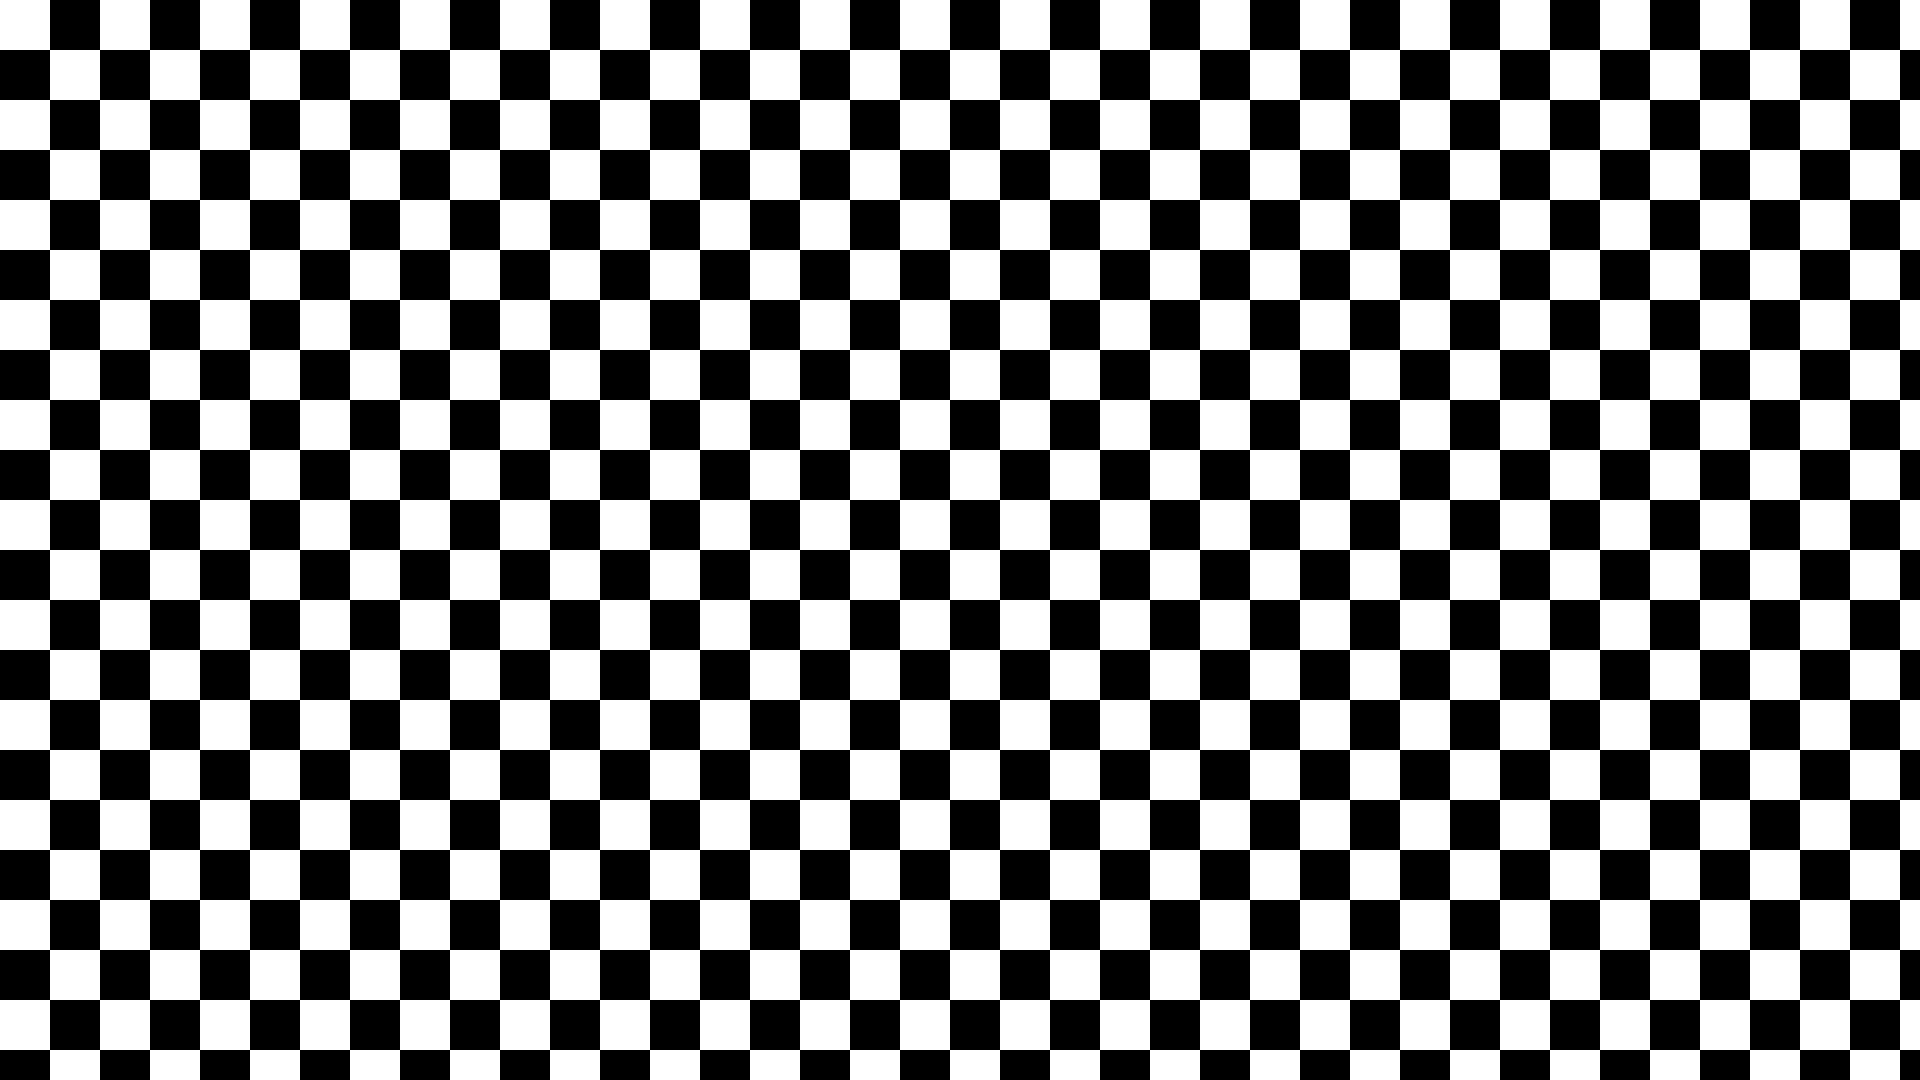
\includegraphics[width=11 cm]{images/calibPattern.png}
 	\end{center}
 	\caption{The calibration pattern.}
 	\label{fig:calibPattern}
 \end{figure}

\subsection{Outputs}
\begin{itemize}
\item a .xml file that we usually name {\tt camera.xml}
\end{itemize}

\subsection{How to Capture Good Images for the Camera Calibration?}
\begin{enumerate}
\item in the software, click in the calibration icon to display the pattern. Do a screenshot and print it.
\item be sure that the printed pattern is not too glossy because specularities make the calibration harder
\item be sure that the calibration pattern is glue over a flat surface and that there is no air bubbles left under the sheet of paper
\item selecting (manually or automatically) the focal length of your camera by taking a sharp image of your object of interest: the object has to be fully visible in this image and not to close to the image edges
\item fix the focal length of your camera by switching the camera to manual (see the physical button of the camera optic)
\item note the distance between the camera and the object: we called it $d_{o \rightarrow c}$
\item take at least 10 different viewpoints of the calibration pattern: check that the images are sharp, that there is no strong specularity in the big part of pattern and that the distance between the pattern and the camera is close to $d_{o \rightarrow c}$. You can take many photos as you want
\end{enumerate}

 \begin{figure}[h]
 	\begin{center}
 		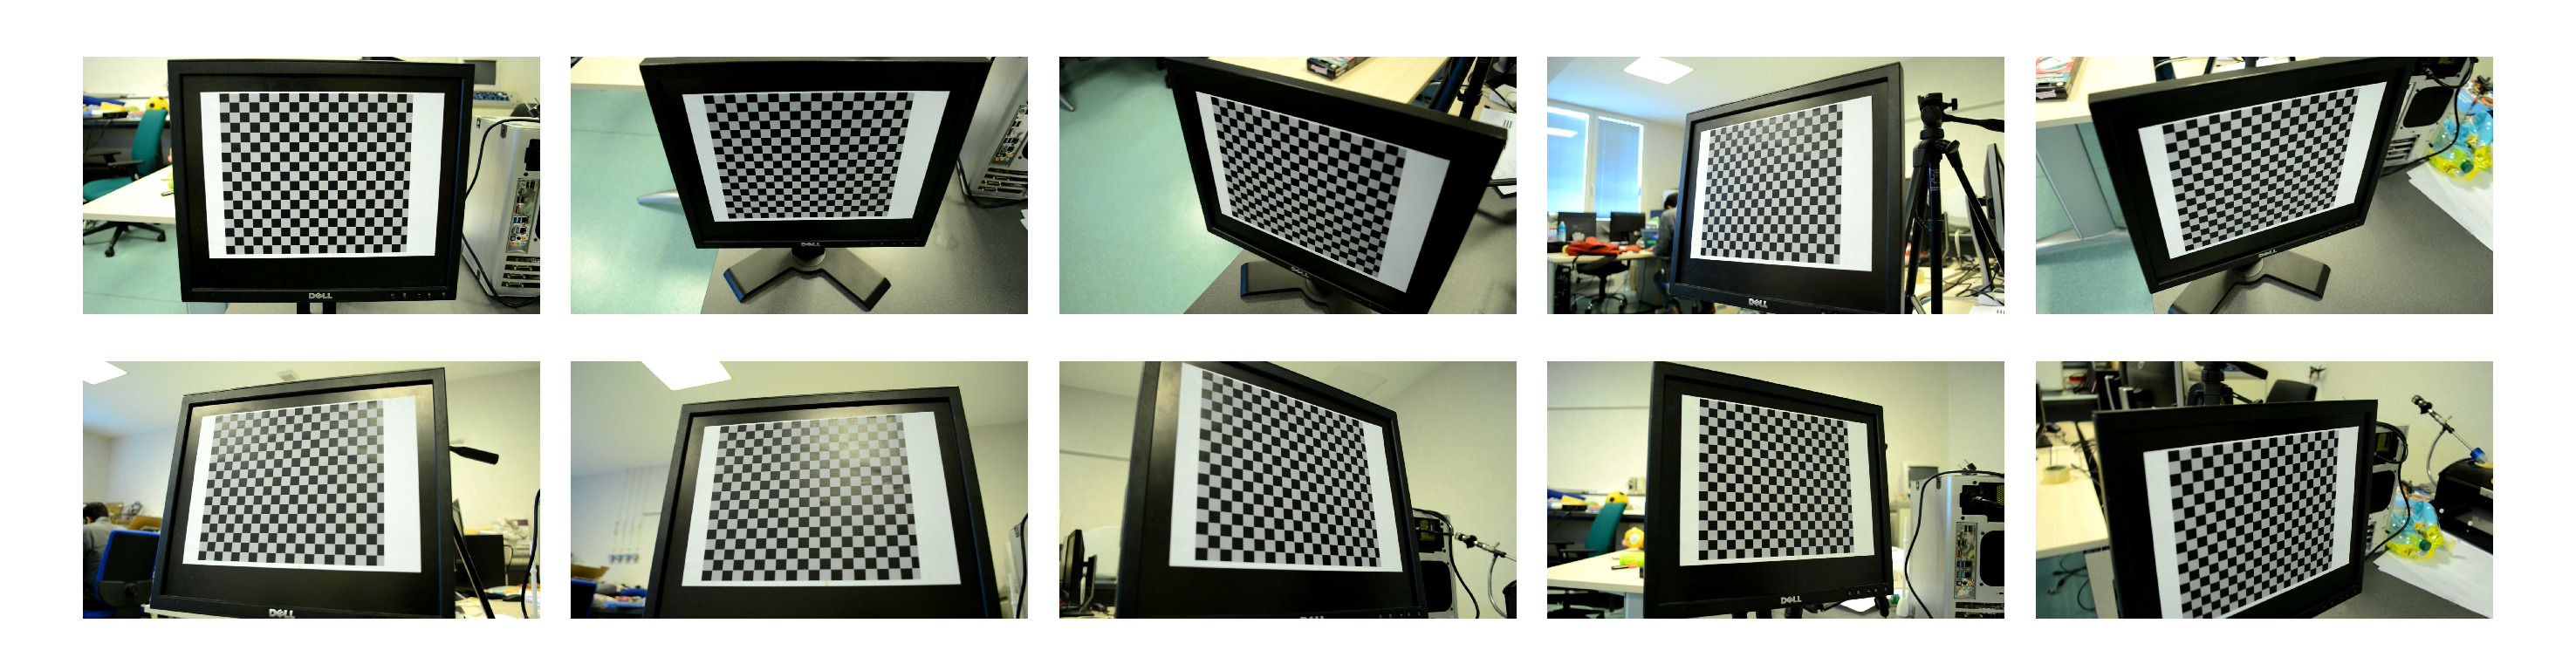
\includegraphics[width=17 cm]{images/calibImages.pdf}
 	\end{center}
 	\caption{Example of calibration images required to perform the camera calibration.}
 	\label{fig:exampleViewpoints}
 \end{figure}

\subsection{General Procedure}
\begin{enumerate}
\item open Agisoft Lens
\item click on Tools $\rightarrow$ Add Photos and select the calibration images
\item click on Tools $\rightarrow$ Calibrate
\item a window such as the figure \ref{fig:calibParamsToEstimate} will appear: select the same calibration parameters
\begin{itemize}
\item the center principal point: cx, cy
\item the radial distorsion parameters: k1, k2, k3
\item the tangential distorsion parameters: p1, p2
\end{itemize}
Note that, with current commercial and industrial cameras, the skew can be assumed to equal to zero and does not need to be estimated.
\item click on Ok: the camera calibration is now being perfomed
\item figure \ref{fig:calibResults} shows the result of camera calibration
\item check if the camera parameters are coherent (see \S\ref{sec:coherentParams})
\item if they are coherent, click on File $\rightarrow$ Save calibration
\end{enumerate}

\subsection{How to Check if the Camera Parameters are Coherent?}
\label{sec:coherentParams}
\begin{itemize}
\item the Image width and height have to be the same as the calibration images
\item the center principal point, x and y, has to be close to the center of the image.

If the value of the principal point is closer to $0$ than half the image size, then you are using a newer version of Agisoft Lens than the one recommended.
Good value of x- and y-components are respectively at $width./2$ $\pm width \times 0.1$  and $height./2$ $\pm height \times 0.1$.
\item the skew has to be equal to zero since we uncheck ``Fit skew''
\item k1, k2 and k3 are the radial distortion parameters.

If the original images do not look to be distorted, k1 has to be less than $0.1$ in absolute value.

If k2 is superior than $100$ in absolute value, verify that the original images are clearly distorted and, if it is not, that means the calibration images do not present enough different viewpoints.

k3 can be superior than $100$ in absolute value. The sign of the radial distortion can be also checked as figure \ref{fig:radialDistortion} indicates.
\item p1 and p2 are the tangential distortion parameters. For the cameras of the lab, p1 and p2 has to smaller than $0.1$.
\item another verification can be done by undistorting the images (see \S\ref{sec:undistort}).
\item do not forget to click on File $\rightarrow$ Save calibration to save the camera parameters.
\end{itemize}

 \begin{figure}[h]
 	\begin{center}
 		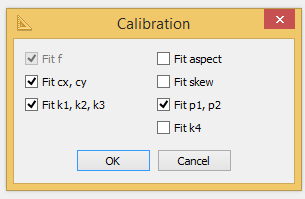
\includegraphics[width=7 cm]{images/calibParamsToSelect.png}
 	\end{center}
 	\caption{Calibration parameters to estimate in Agisoft Lens.}
 	\label{fig:calibParamsToEstimate}
 \end{figure}

 \begin{figure}[h]
 	\begin{center}
 		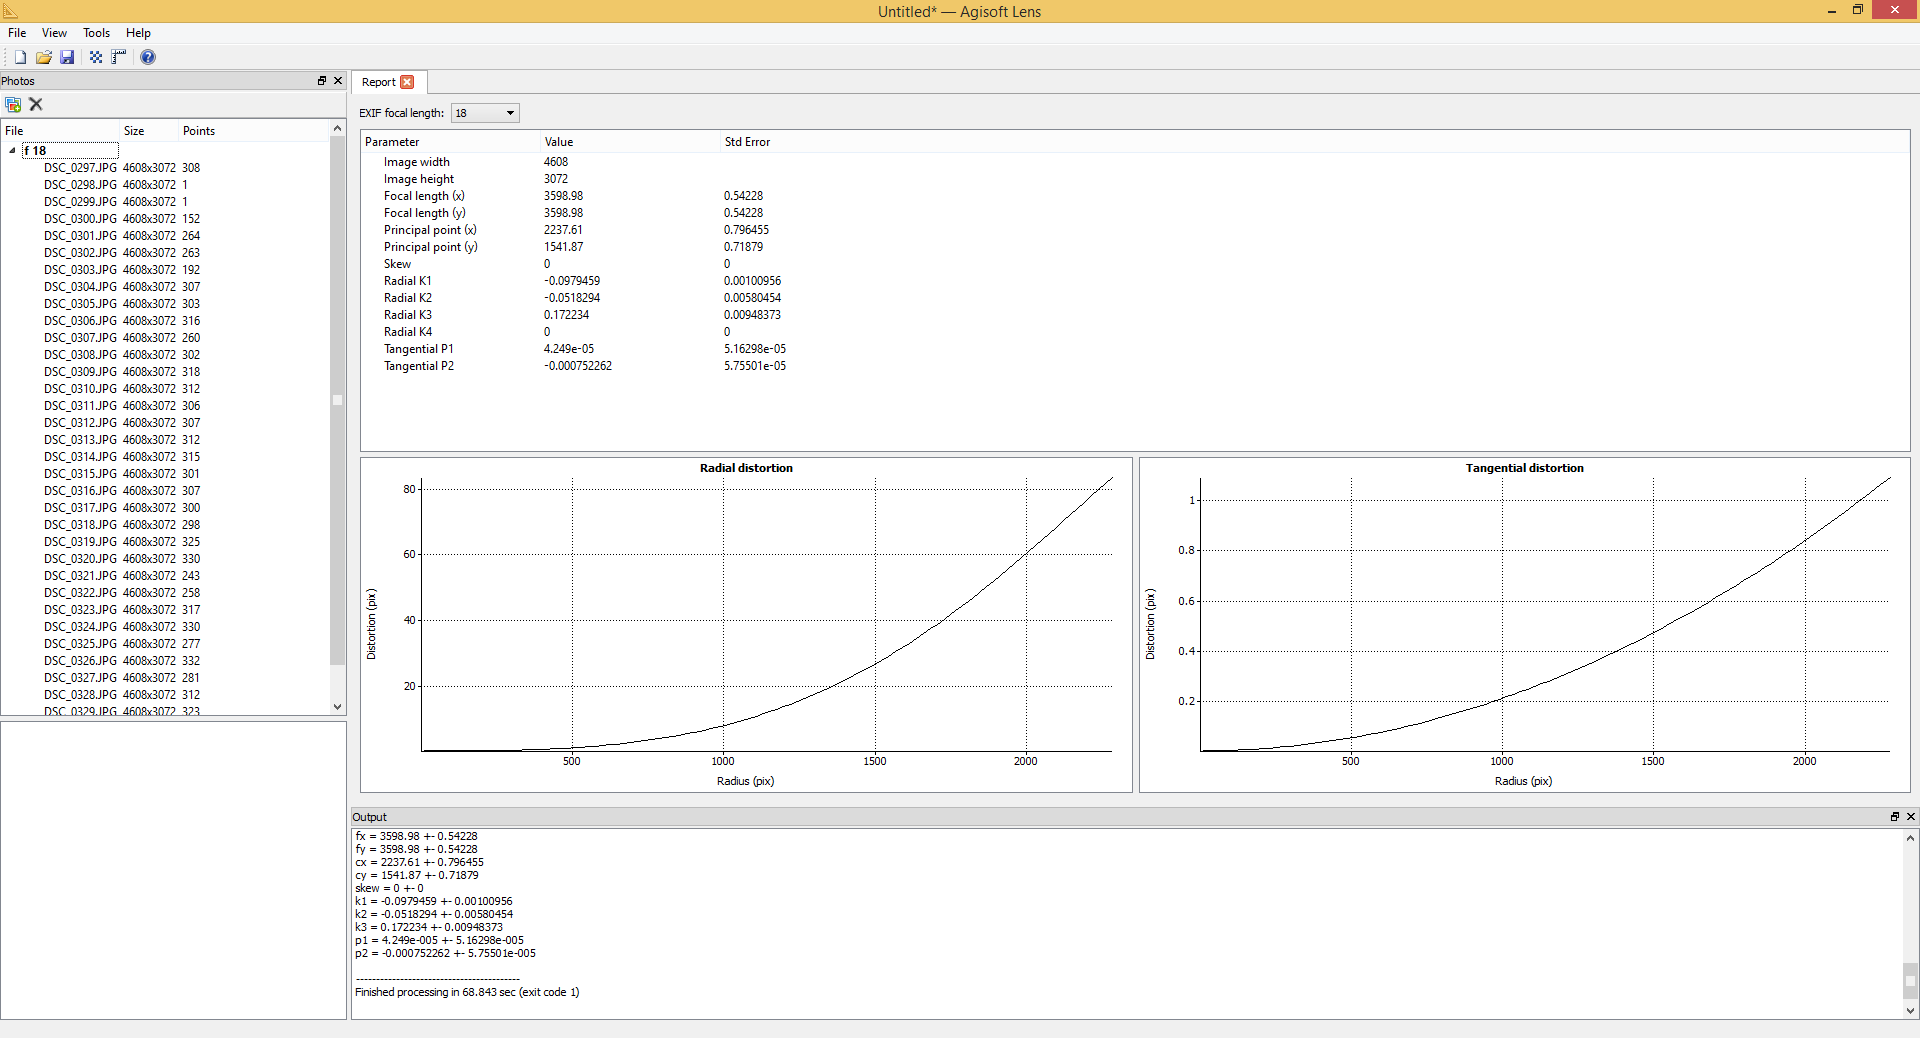
\includegraphics[width=17 cm]{images/resultsLens.png}
 	\end{center}
 	\caption{Results of camera calibration.}
 	\label{fig:calibResults}
 \end{figure}
 
  \begin{figure}[h]
 	\begin{center}
 		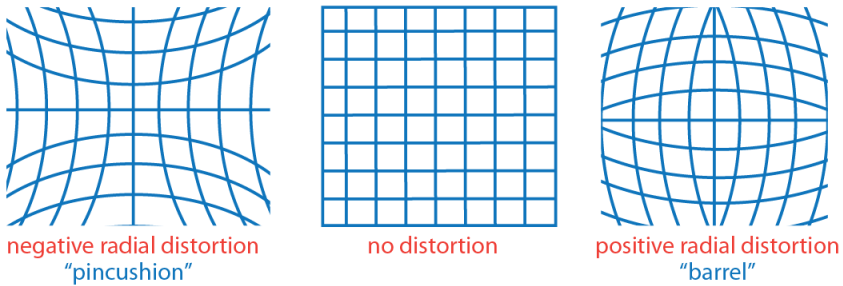
\includegraphics[width=10 cm]{images/cameracalibrator_radial.png}
 	\end{center}
 	\caption{Relationship between the sign of radial distorsion parameters and its visual effect. Source: \cite{radialDistortion}.}
 	\label{fig:radialDistortion}
 \end{figure}


\section{3D Reconstruction Using SfM: Agisoft PhotoScan}
\subsection{Which versions?}
We recommend to choose the following version: v 1.2.6 (2331 build).
The reason is that the data format of the camera calibration from Agisoft Lens is readable by this version.
Older versions are also good.
\subsection{Inputs}
\begin{itemize}
\item a set of images of the object of interest in a rigid pose all over the sequence. The number of images can vary depending on the complexity of the surface and its texture. See \S\ref{sec:takingObjectPictures} for tips to acquire pictures which lead to good 3D reconstructions.
\item the camera calibration file {\tt camera.xml} of the camera which is used to take the set of object images.
\end{itemize}
\subsection{Outputs}
\begin{itemize}
\item a 3D texture-mapped model of the object of interest contained in 3 files {\tt .obj}, {\tt .mtl} and {\tt .png} ( or {\tt .tif})
\item the extrinsic camera parameters that we name {\tt PSCameras.xml}. It contains the rigid transformation (rotation and translation) between the world coordinates frame and each camera coordinates frame, which corresponds to each object image.
\item the masks of each image to extract the foreground from the background
\item the undistorted images used to do the 3D reconstruction
\end{itemize}

\subsection{How to Capture Good Images for the 3D Reconstruction?}
\label{sec:takingObjectPictures}
There are already good manuals on internet. In the folder {\tt ./docs} attached to this report, you will find \citep{photoscanDocs} and another document with some similar informations.
The \textit{Chapter 2. Capturing photos} of \citep{photoscanDocs} provides useful information.
Here we provide some information that we found relevant for our works.
There is no theoretical conditions.
Therefore, one has to train his intuition to know a priori when an object will be correctly reconstructed.

\subsubsection{Problem 1: When the Object Surface is Well-Textured, but When the Texture is Repetitive and the Shape is Symmetric}
\paragraph{Problem}
This scenario can make the reconstruction impossible or wrong. The figure \ref{fig:wellText_pb} shows two examples of ambiguous objects and shapes.
Both sides are not enough different, but each of them is sufficiently well-textured to obtain a 3D reconstruction of one side.
Therefore, it is possible to reconstruct each side separately, but, if we align the pictures of both sides, we will see that the solution proposed is just one face.
This is due to the fact that the texture and the shape of both sides are not enough different.

  \begin{figure}[h]
 	\begin{center}
 		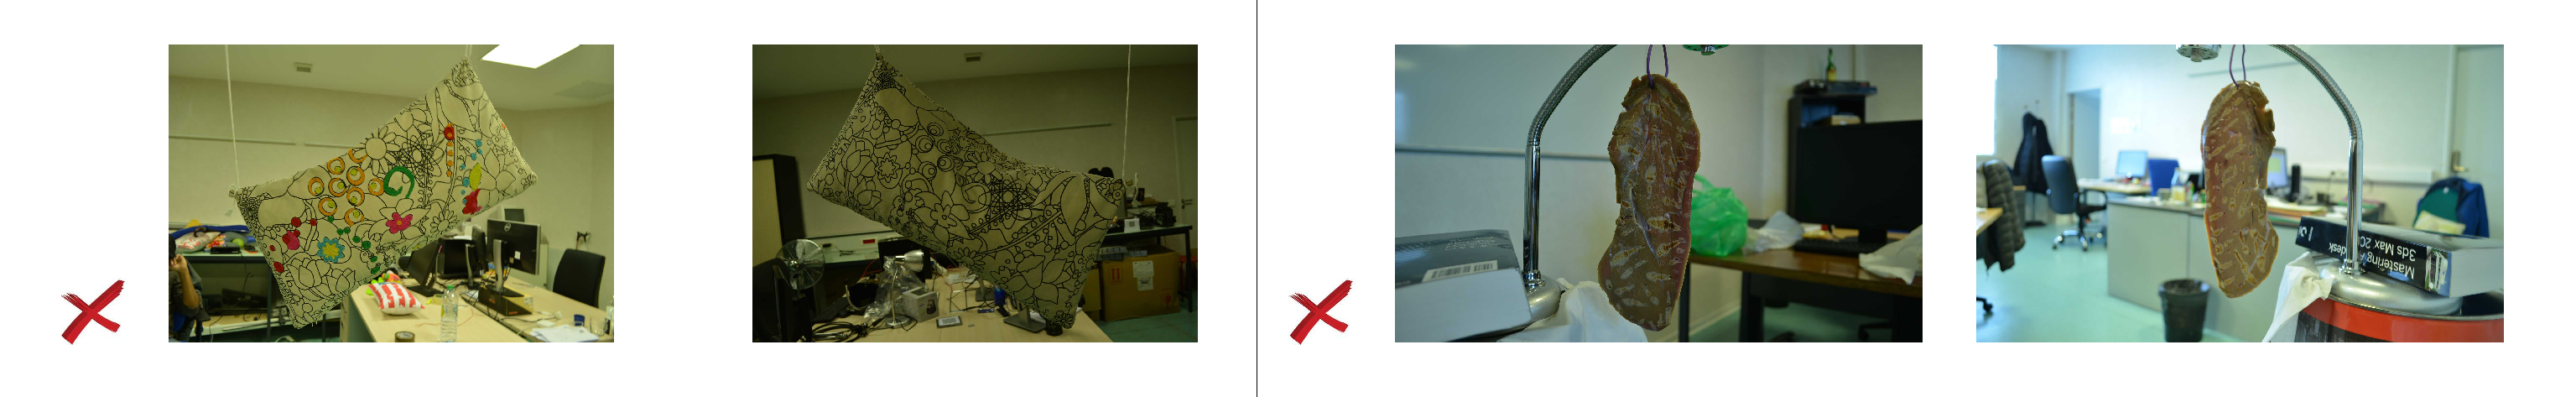
\includegraphics[width=17 cm]{images/wellText_pb.pdf}
 	\end{center}
 	\caption{Examples of ambiguous object shapes. Both sides are quite similar and the shape is not enough discriminative.}
 	\label{fig:wellText_pb}
 \end{figure}


\paragraph{Solution}
Figure \ref{fig:wellText_sol} illustrates some solutions to this issue.
These new sequences lead to good reconstructions.
\begin{itemize}
\item make the texture very different between all the sides
\item place the object (if the object is deformable) such that the shape is not too symmetric
\end{itemize}

  \begin{figure}[h]
 	\begin{center}
 		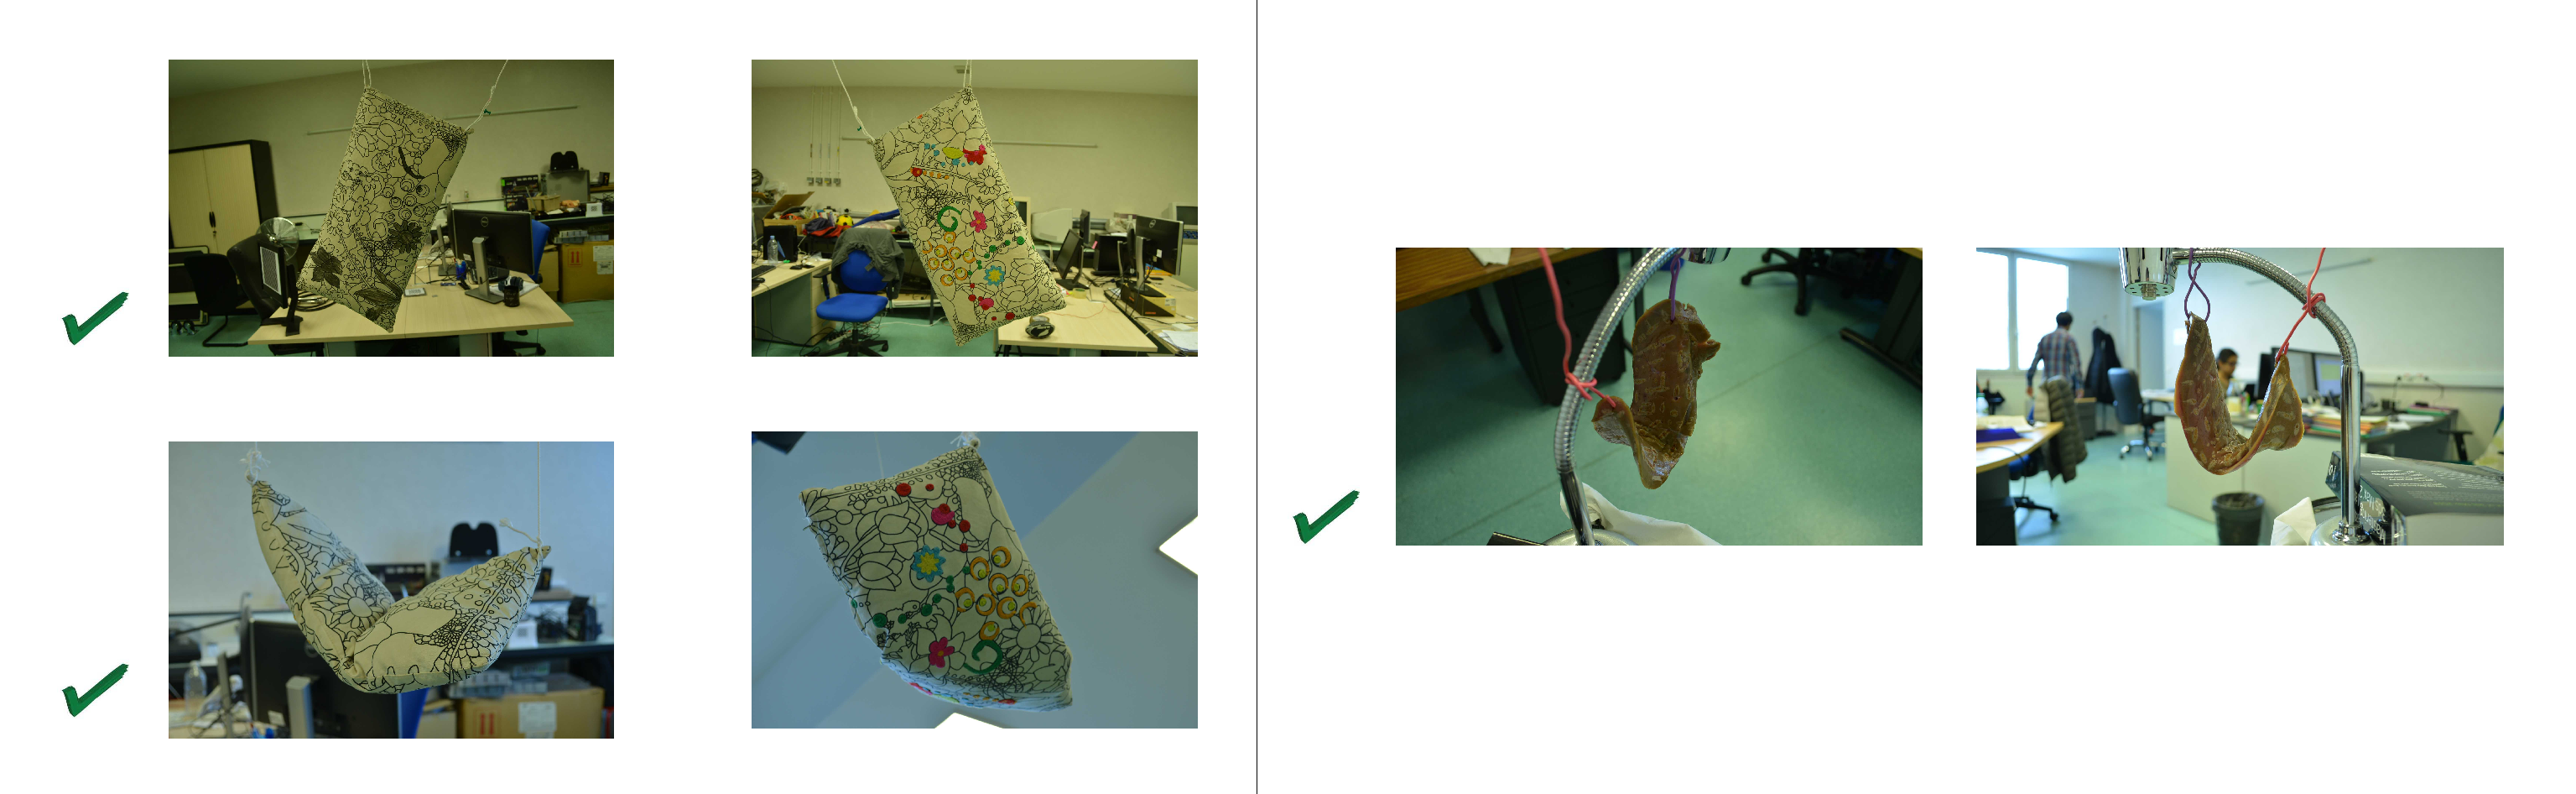
\includegraphics[width=17 cm]{images/wellText_sol.pdf}
 	\end{center}
 	\caption{Examples of good shapes that lead to a good reconstruction.}
 	\label{fig:wellText_sol}
 \end{figure}

\subsubsection{Problem 2: When the Object Surface is Poorly-Textured}
\paragraph{Problem}
In this scenario, the object is not enough textured.
This makes the reconstruction very difficult even impossible. 

\paragraph{Solution}
\begin{itemize}
\item add texture all over the surface
\item do not use masks and capture the pictures with a textured background.
In deed, a textured background can be very beneficial for this case since it provides more constraints for the reconstruction.
However, be sure that the background does not change during the sequence.
\end{itemize}

\subsection{Procedure}
A good tutorial to perform 3D reconstruction with Agisoft PhotoScan is provided in this following link:
\url{http://www.agisoft.com/pdf/PS_1.1%20-Tutorial%20(IL)%20-%203D-model.pdf}.

\subsection{Good practices}
\begin{itemize}
\item save the project as soon as possible
\item save as soon as possible the masks in a folder named {\tt ./masks} because segmenting the images takes time and has to be done again if the software crashes
\end{itemize}

\subsection{How to Undistort Images from Agisoft PhotoScan?}
\label{sec:undistort}
\begin{enumerate}
\item open Agisoft Lens
\item click on Workflow $\rightarrow$ Add Photos and select the images to undistort
\item click on Tools $\rightarrow$ Camera Calibration
\item load you camera calibration file {\tt camera.xml} and check ``Fix Calibration'' (so Agisoft PhotoScan cannot change the camera parameters)
\item click on Tools $\rightarrow$ Export $\rightarrow$ Undistort Photos: figure \ref{fig:undistortPhotos} will appear
\item be sure that the box of ``Center principal'' point is unchecked such as the figure \ref{fig:undistortPhotos} shows
\item click on ``OK'' and select a folder to store the undistorted images
\end{enumerate}

  \begin{figure}[h]
 	\begin{center}
 		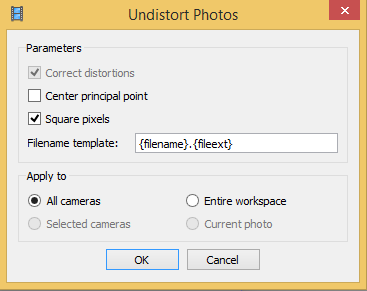
\includegraphics[width=8 cm]{images/undistortPhotos_PS.png}
 	\end{center}
 	\caption{The options window to undistort the images in Agisoft PhotoScan.}
 	\label{fig:undistortPhotos}
 \end{figure}

%\section{Preparing Ground-Truth Data using Matlab Codes}
%
%\subsection{Extracting Intrinsic and Extrinsic Camera Parameters}
%
%In the folder ``codes'', you will find the code \texttt{.m} which extracts the camera data from the Agisoft Lens format and outputs the camera data in easier format to work on Matlab.
%
%\subsection{Using a Motion-Based SfT Method}
%
%
%
%  \begin{figure}[h]
% 	\begin{center}
% 		\includegraphics[width=17 cm]{images/usingSfT.pdf}
% 	\end{center}
% 	\caption{The options window to undistort the images in Agisoft PhotoScan.}
% 	\label{fig:usingSfT}
% \end{figure}
% 
%\subsection{Validating a Motion-Based SfT Method}
%
%  \begin{figure}[h]
% 	\begin{center}
% 		\includegraphics[width=17 cm]{images/validatingSfT.pdf}
% 	\end{center}
% 	\caption{The options window to undistort the images in Agisoft PhotoScan.}
% 	\label{fig:validatingSfT}
% \end{figure}
%
\bibliographystyle{abbrvnat}
\bibliography{biblio}

\end{document}



